%
%==> Section: Putting labels in pictures
%
\section{
  Putting labels in pictures
}

\begin{frame}[fragile]
  \frametitle{
    Putting labels in pictures
}

  When you construct a picture, in 99\% of cases you also need to put labels. This is easy! Let us start by seeing how we would place some text in a picture.

  \lstinputlisting{./tex/src/put_text_in_pictures.tex}
  
  yields

  \begin{center}
    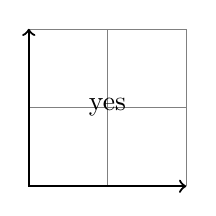
\begin{tikzpicture}
  \draw [help lines] (0,0) grid (2,2);
  \draw [thick, <->] (0,2) -- (0,0) -- (2,0);
  \node at (1,1) {yes};
\end{tikzpicture}

  \end{center}

 Notice how the ``yes" is positioned: the center of its ``baseline" is at $(1,1).$

\end{frame}

%
%==> Relative positioning 
%
\begin{frame}[fragile]
  \frametitle{
    Relative positioning
  }

  Sometimes you want a label to be situated relative to a point. Ti$k$Z has neat
  commands for this. For instance you can write

  \lstinputlisting{./tex/src/relative_positioning.tex}
  
  to get

  \begin{center}
    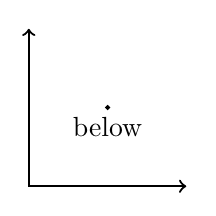
\begin{tikzpicture}
  \draw [thick, <->] (0,2) -- (0,0) -- (2,0);
  \draw[fill] (1,1) circle [radius=0.025];
  \node [below] at (1,1) {below};
\end{tikzpicture}

    \end{center}

\end{frame}

%
%==> More relative positioning
%
\begin{frame}[fragile]

  You are not limited to put things below a point:

  \lstinputlisting{./tex/src/more_relative_positioning.tex}
  
  yields
  
  \begin{center}
    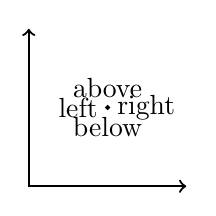
\begin{tikzpicture}
  \draw [thick, <->] (0,2) -- (0,0) -- (2,0);
  \draw [fill] (1,1) circle [radius=0.025];
  \node [below] at (1,1) {below};
  \node [above] at (1,1) {above};
  \node [left] at (1,1) {left};
  \node [right] at (1,1) {right};
\end{tikzpicture}

  \end{center}

\end{frame}
%
%==> Mix and match positioning
%
\begin{frame}[fragile]
  
  And, you can also mix and match

  \lstinputlisting{./tex/src/mix_and_match_positioning.tex}
  
  yields

  \begin{center}
    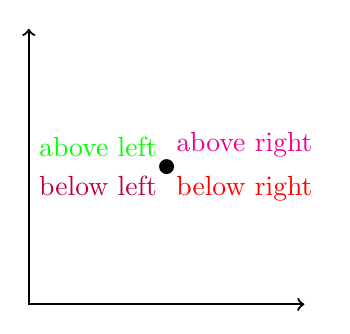
\begin{tikzpicture}[scale=3.5]
  \draw [thick, <->] (0,1) -- (0,0) -- (1,0);
  \draw[fill] (.5,.5) circle [radius=0.025];
  \node [below right, red] at (.5,.5) {below right};
  \node [above left, green] at (.5,.5) {above left};
  \node [below left, purple] at (.5,.5) {below left};
  \node [above right, magenta] at (.5,.5) {above right};
\end{tikzpicture}

  \end{center}

\end{frame}

%
%==> Labeling axes and points
%
\begin{frame}[fragile]
  \frametitle{
    Labeling axes and points
  }

  \lstinputlisting{./tex/src/label_axes_and_points.tex}
  
  gives us
  
  \begin{center}
    \begin{tikzpicture}[xscale=3, yscale=1.5]
  \draw [thick, <->] (0,1) -- (0,0) -- (1,0);
  \node [below right] at (1,0) {$x$};
  \node [left] at (0,1) {$y$};
  \draw [fill] (.4,.6) circle [radius=.5pt];
  \node[above right] (.4,.6) {$A$};
\end{tikzpicture}

  \end{center}

\end{frame}

%
%==> Supressing \node
%
\begin{frame}[fragile]

  You can avoid some typing by mixing nodes in the middle of paths. For instance the last figure could have been written as follows:

  \lstinputlisting{./tex/src/label_axes_and_points_alt.tex}
  
  which would have given exactly the same result. Note that the node is put after the point to which it is attached and that we suppress the $\backslash$ in

  \begin{lstlisting}
    \node
  \end{lstlisting}
  

\end{frame}

%
%==> Fancy nodes
%
\begin{frame}[containsverbatim]
  \frametitle{
    Fancy nodes
  }

  You may want to put several lines in your ``node" (this is convenient when drawing time lines for instance). This can be done by using the standard \LaTeX\, for indicating a new line but you must tell Ti$k$Z how to align things. From

  {
    \scriptsize
    \lstinputlisting{./tex/src/fancy_nodes.tex}
  }
  
  we obtain

  \begin{center}
    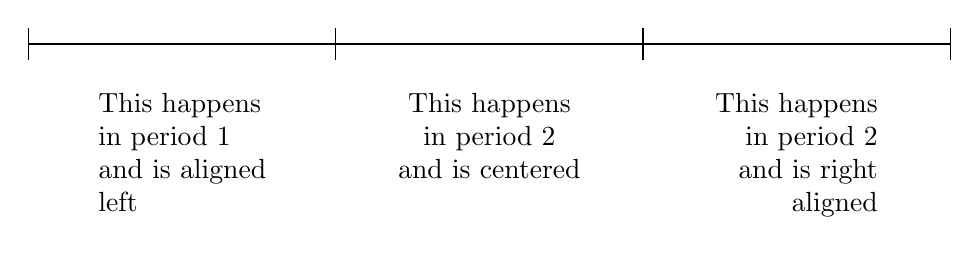
\begin{tikzpicture}[xscale=1.3]
  \draw [thick] (0,0) -- (9,0);
  \draw (0,-.2) -- (0, .2);
  \draw (3,-.2) -- (3, .2);
  \draw (6,-.2) -- (6, .2);
  \draw (9,-.2) -- (9, .2);
  \node[align=left, below] at (1.5,-.5)%
       {This happens\\in period 1\\and is aligned\\ left};
  \node[align=center, below] at (4.5,-.5)%
       {This happens\\in period 2\\and is centered};
  \node[align=right, below] at (7.5,-.5)%
       {This happens\\in period 2\\and is right\\aligned};
\end{tikzpicture}

  \end{center}
  
\end{frame}
